\documentclass[10pt]{article}
\usepackage[ngerman]{babel}
\usepackage[utf8]{inputenc}
\usepackage[T1]{fontenc}
\usepackage{amsmath}
\usepackage{amsfonts}
\usepackage{amssymb}
\usepackage[version=4]{mhchem}
\usepackage{stmaryrd}
\usepackage{graphicx}
\usepackage[export]{adjustbox}
\graphicspath{ {./images/} }
\usepackage{bbold}

\title{Hauptprüfung Abiturprüfung 2023 - Leistungsfach }

\author{Alexander Schwarz\\
www.mathe-aufgaben.com}
\date{}


\begin{document}
\maketitle
 Baden-Württemberg

\section*{Aufgabe A 2.1 (14,5 VP)}
Die Abbildung stellt die Planskizze einer Landstraße dar. Der Verlauf dieser Landstraße wird durch den Graphen der Funktion $f$ mit $f(x)=\frac{3}{8} x^{3}-\frac{27}{8} x^{2}+9 x-\frac{13}{2}$ für $0 \leq x \leq \frac{9}{2}$ beschrieben. Die positive y-Achse beschreibt dabei die Himmelsrichtung Norden, die positive x-Achse die Himmelsrichtung Osten. Eine Längeneinheit im Koordinatensystem entspricht einem Kilometer in der Realität.\\
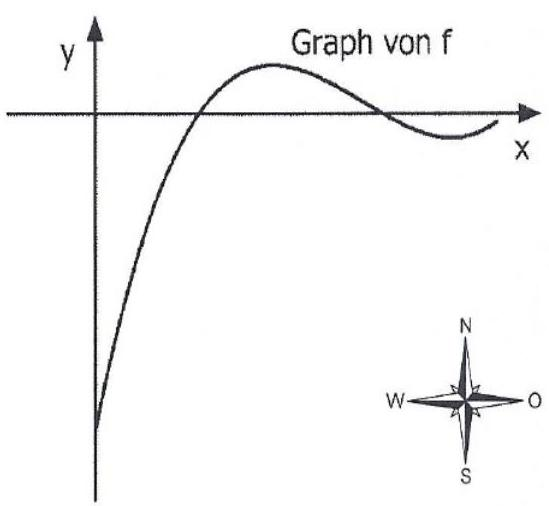
\includegraphics[max width=\textwidth, center]{2025_04_24_6c638485c3c5bdc20e69g-2}\\
a) Bestimmen Sie die Koordinaten des Punkts P , der den nördlichsten Punkt der Landstraße darstellt.\\
(2,5 VP)\\
An der Stelle $\mathrm{x}_{0}=3$ wechselt das Vorzeichen der Funktion f" vom Negativen ins Positive. Beschreiben Sie, was dies für den Verlauf der Landstraße bedeutet. (Teilergebnis: $\mathrm{P}(2 \mid 1)$ )\\
(1 VP)\\
b) Ein Teil des Graphen der Funktion $g$ mit $g(x)=-\frac{27}{8} x^{2}+\frac{75}{8} x-\frac{13}{2}$ stellt einen

Fahrradweg dar, der zwei Punkte der Landstraße verbindet. Diese beiden Punkte werden durch $A(a \mid f(a))$ und $B(b \mid f(b))$ mit $a<b$ dargestellt.\\
Bestimmen Sie die Koordinaten von A und B .\\
(Teilergebnis: $a=0$ und $b=1$ )\\
Berechnen Sie $\int_{0}^{1}(g(x)-f(x)) d x$ und interpretieren Sie das Ergebnis im\\
Sachzusammenhang.\\
(2,5 VP)

Im Folgenden wird auch der Höhenverlauf der Landstraße betrachtet. Stellt $\mathrm{R}(\mathrm{r} \mid \mathrm{f}(\mathrm{r})$ ) einen Punkt auf der Landstraße dar, so gilt für seine Höhe h(r):

$$
h(r)=u(f(r)) \text { mit } u(x)=2-\frac{1}{500}(x-1)^{2}
$$

$(h(r)$ in Kilometer über der Meereshöhe)\\
c) Zeigen Sie, dass der westlichste Punkt der Landstraße auf einer Höhe von etwa 1890 Meter liegt.\\
(1,5 VP)\\
Begründen Sie, dass kein Punkt der Landstraße höher als 2000 Meter liegt.\\
(1,5 VP)\\
Der am höchsten gelegene Punkt auf der Landstraße wird durch den Punkt S auf dem Graphen von f dargestellt. Bestimmen Sie die Koordinaten von S.\\
d) Zum Abfluss von Regenwasser sind die durch $\mathrm{P}(2 \mid 1)$ und $\mathrm{Q}(0 \mid \mathrm{f}(0))$ dargestellten Punkte auf der Landstraße durch ein geradlinig verlaufendes Rohr verbunden. Berechnen Sie das Gefälle dieses Rohrs.

\section*{Aufgabe A 2.2 (5,5 VP)}
Für jedes $a \in \mathbb{R}$ ist eine Funktion $f_{a}$ gegeben durch $f_{a}(x)=\sin \left(\frac{\pi}{a^{2}+1} \cdot x\right)$ -\\
Die zugehörigen Graphen werden mit $\mathrm{G}_{\mathrm{a}}$ bezeichnet.\\
a) Berechnen Sie die Größe des Steigungswinkels der Tangente an $G_{0}$ im Ursprung.\\
b) Bestimmen Sie denjenigen Wert von a, für den die Periode von $f_{a}$ minimal wird.\\
c) Die Tangente an $G_{a}$ an der Stelle $x_{0}=0$ und die Tangente an $G_{a}$ an der kleinsten positiven Nullstelle von $f_{a}$ schließen mit der x-Achse ein Dreieck ein. Bestimmen Sie alle Werte von a, für die der Inhalt dieses Dreiecks $2,5 \pi$ beträgt. (3 VP)

\section*{Lösungen}
\section*{Aufgabe A 2.1}
a) Bestimmen Sie die Koordinaten des Punkts P, der den nördlichsten Punkt der Landstraße darstellt.

Der nördlichste Punkt ist der Hochpunkt des Schaubildes von f.\\
Notwendige Bedingung für Hochpunkt: $f^{\prime}(x)=0$\\
$f(x)=\frac{3}{8} x^{3}-\frac{27}{8} x^{2}+9 x-\frac{13}{2}$\\
$f^{\prime}(x)=\frac{9}{8} x^{2}-\frac{27}{4} x+9$\\
$\frac{9}{8} x^{2}-\frac{27}{4} x+9=0 \quad|\cdot 8 \quad|: 9$\\
$x^{2}-6 x+8=0$\\
abc-Formel: $x_{1,2}=\frac{6 \pm \sqrt{36-32}}{2}=\frac{6 \pm 2}{2} \quad x_{1}=4$ und $x_{2}=2$\\
Anhand der Abbildung ist zu erkennen, dass der Hochpunkt bei $x=2$ vorliegt. Mit $f(2)=1$ lautet der gesuchte Punkt $P(2 \mid 1)$.

Beschreiben Sie, was dies für den Verlauf der Landstraße bedeutet.\\
Die zweite Ableitungsfunktion beschreibt die Krümmung des Schaubildes von f. An der Stelle x = 3 existiert eine Wendestelle, das heißt es findet dort ein Krümmungswechsel statt.\\
Für $\mathrm{x}<3$ ist das Schaubild von f rechtsgekrümmt und für $\mathrm{x}>3$ linksgekrümmt.\\
b) Bestimmen Sie die Koordinaten von $A$ und $B$.

Die Punkte A und B sind die Schnittpunkte der Schaubilder von f und g.\\
Bedingung: $f(x)=g(x)$\\
$\frac{3}{8} x^{3}-\frac{27}{8} x^{2}+9 x-\frac{13}{2}=-\frac{27}{8} x^{2}+\frac{75}{8} x-\frac{13}{2}$\\
$\Leftrightarrow \frac{3}{8} x^{3}-\frac{3}{8} x=0 \Leftrightarrow x \cdot\left(\frac{3}{8} x^{2}-\frac{3}{8}\right)=0 \quad$ Lösung mit dem Satz vom Nullprodukt\\
Gleichung I): $x=0$\\
Gleichung II): $\frac{3}{8} x^{2}-\frac{3}{8}=0 \Leftrightarrow x^{2}=1 \Leftrightarrow x= \pm 1$\\
Da $0 \leq x \leq \frac{9}{2}$ gelten soll, fällt die Lösung $x=-1$ weg.

Mit $g(0)=-\frac{13}{2}$ ergibt sich Punkt $A\left(0 \left\lvert\,-\frac{13}{2}\right.\right)$\\
Mit $\mathrm{g}(1)=-0,5$ ergibt sich Punkt $\mathrm{B}(1 \mid-0,5)$\\
Berechnen Sie $\int_{0}^{1}(g(x)-f(x)) d x$ und interpretieren Sie das Ergebnis im Sachzusammenhang.\\
$\int_{0}^{1}(g(x)-f(x)) d x=\int_{0}^{1}\left(-\frac{27}{8} x^{2}+\frac{75}{8} x-\frac{13}{2}-\left(\frac{3}{8} x^{3}-\frac{27}{8} x^{2}+9 x-\frac{13}{2}\right)\right) d x$ $=\int_{0}^{1}\left(\frac{3}{8} x-\frac{3}{8} x^{3}\right) d x=\left[\frac{3}{16} x^{2}-\frac{3}{32} x^{4}\right]_{0}^{1}=\frac{3}{16}-\frac{3}{32}-0=\frac{3}{32}=0,09375$

Interpretation:\\
Der Inhalt der Fläche, die von der Landstraße und dem Fahrradweg begrenzt wird, beträgt $0,09375 \mathrm{~km}^{2}$.\\
c) Zeigen Sie, dass der westlichste Punkt der Landstraße auf einer Höhe von etwa 1890 Meter liegt.

Für den westlichsten Punkt der Landstraße gilt $\mathrm{x}=0$ und somit $\mathrm{r}=0$.\\
$h(0)=u(f(0))=u\left(-\frac{13}{2}\right)=2-\frac{1}{500}\left(-\frac{13}{2}-1\right)^{2}=1,8875 \mathrm{~km}$\\
Damit liegt der Punkt auf etwa 1890 m Höhe.\\
Begründen Sie, dass kein Punkt der Landstraße höher als 2000 Meter liegt.\\
Hier muss man die äußere Funktion $u(x)$ untersuchen.\\
Aus der Funktionsgleichung $u(x)=2-\frac{1}{500}(x-1)^{2}$ ergibt sich $u(x) \leq 2$, da der Term $\frac{1}{500}(x-1)^{2} \geq 0$ ist.

Da die Funktion $\mathrm{u}(\mathrm{x})$ einen Funktionswert größer als 2 nicht annehmen kann, kann auch kein Punkt höher als 2000 m liegen.

Bestimmen Sie die Koordinaten von S.\\
Die größte Höhe wird für $x=1$ erreicht, da die Funktion u für $x=1$ maximal wird. (Das Schaubild von u ist eine nach unten geöffnete Parabel mit dem Scheitelpunkt (1|2)).

Da $u(1)=2$ gilt und weil der $x$-Wert von $u$ dem $y$-Wert von $f$ entspricht (verkettete Funktion) folgt daraus als Bedingung $f(x)=1$

Da in a) der Punkt $P(2 \mid 1)$ als Hochpunkt des Schaubildes von $f$ berechnet wurde und den geforderten y-Wert 1 besitzt, entspricht $S$ dem Punkt $P$, also $S(2 \mid 1)$.\\
d) Berechnen Sie das Gefälle dieses Rohrs.

Um das Gefälle zu berechnen, benötigt man zunächst den Höhenunterschied der Landstraßenpunkte $\mathrm{P}(2 \mid 1)$ und $\mathrm{Q}(0 \mid \mathrm{f}(0))$.

Höhe bei P: $h(2)=u(f(2))=u(1)=2$\\
Höhe bei $Q$ : $h(0)=u(f(0))=u\left(-\frac{13}{2}\right)=1,8875$\\
Höhenunterschied $=0,1125 \mathrm{~km}$\\
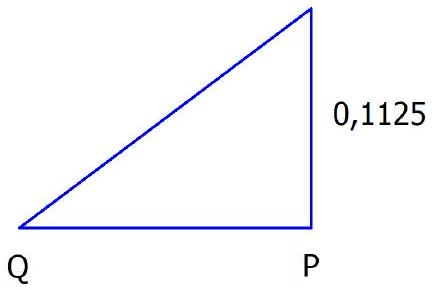
\includegraphics[max width=\textwidth, center]{2025_04_24_6c638485c3c5bdc20e69g-6}

Abstand von $\mathrm{P}(2 \mid 1) \mathrm{zu} \mathrm{Q}\left(0 \left\lvert\,-\frac{13}{2}\right.\right):|\overrightarrow{\mathrm{PQ}}|=\left|\binom{-2}{-7,5}\right|=\sqrt{4+56,25}=\sqrt{60,25}$ Gefälle $=\frac{0,1125}{\sqrt{60,25}} \approx 0,014=1,4 \%$

\section*{Aufgabe A 2.2}
e) Berechnen Sie die Größe des Steigungswinkels der Tangente an $G_{0}$ im Ursprung.\\
$\mathrm{f}_{0}(\mathrm{x})=\sin (\pi \cdot \mathrm{x})$\\
Es gilt $\mathrm{f}_{0}^{\prime}(\mathrm{x})=\cos (\pi \cdot x) \cdot \pi$\\
Steigung der Tangente im Ursprung: $\mathrm{f}_{0}^{\prime}(0)=\cos (0) \cdot \pi=\pi$\\
Steigungswinkel: $\tan (\alpha)=\pi \Rightarrow \alpha=\tan ^{-1}(\pi)=72,3^{\circ}$\\
b) Bestimmen Sie denjenigen Wert von a, für den die Periode von $\mathrm{f}_{\mathrm{a}}$ minimal wird.

Die Periode ist $p_{a}=\frac{2 \pi}{\pi / a^{2}+1}=2\left(a^{2}+1\right)$\\
Dier Periode wird minimal für $\mathrm{a}=0$.\\
c) Bestimmen Sie alle Werte von a, für die der Inhalt dieses Dreiecks $2,5 \pi$ beträgt.

Die kleinste positive Nullstelle befindet sich nach einer halben Periode.\\
Da die Periode $p_{a}=2\left(a^{2}+1\right)$ beträgt, ist die gesuchte Nullstelle $x=a^{2}+1$\\
Zwei Eckpunkte des Dreiecks sind $P(0 \mid 0)$ und $Q_{a}\left(a^{2}+1 \mid 0\right)$.\\
Gleichung der Tangente an der Stelle $x=0$ :\\
Tangentenformel: $y=f_{a}^{\prime}(0) \cdot(x-0)+f_{a}(0)$\\
Wegen $f_{a}^{\prime}(x)=\cos \left(\frac{\pi}{a^{2}+1} x\right) \cdot \frac{\pi}{a^{2}+1}$ folgt $f_{a}^{\prime}(0)=\frac{\pi}{a^{2}+1}$.\\
Außerdem gilt $f_{a}(0)=0$.\\
Tangentengleichung: $y=\frac{\pi}{a^{2}+1} \cdot(x-0)+0 \Leftrightarrow y=\frac{\pi}{a^{2}+1} \cdot x$\\
Aus Symmetriegründen schneiden sich die beiden Tangenten in der Mitte der beiden Nullstellen, also an der Stelle $x=\frac{0+a^{2}+1}{2}=\frac{a^{2}+1}{2}$\\
Einsetzen des $x$-Wertes in die Tangentengleichung: $y=\frac{\pi}{a^{2}+1} \cdot \frac{a^{2}+1}{2}=\frac{\pi}{2}$.\\
Der dritte Eckpunkt des Dreiecks lautet $R_{a}\left(\left.\frac{a^{2}+1}{2} \right\rvert\, \frac{\pi}{2}\right)$.\\
Flächeninhalt des Dreiecks: $A_{a}=\frac{1}{2} \cdot \overline{P Q_{a}} \cdot \frac{\pi}{2}=\frac{1}{2} \cdot\left(a^{2}+1\right) \cdot \frac{\pi}{2}=\frac{\pi}{4}\left(a^{2}+1\right)$\\
Bedingung: $\frac{\pi}{4}\left(a^{2}+1\right)=2,5 \pi \Leftrightarrow a^{2}+1=10 \Leftrightarrow a= \pm 3$


\end{document}